\documentclass{beamer}
\usepackage[utf8]{inputenc}
\usepackage{graphicx, epsfig}
\usepackage{amsmath,mathrsfs,amsfonts,amssymb}
\usepackage{floatflt}
\usepackage{epic,ecltree}
\usepackage{mathtext}
\usepackage{fancybox}
\usepackage{fancyhdr}
\usepackage{multirow}
\usepackage{enumerate}
\usepackage{epstopdf}
\usepackage{multicol}
\usepackage{algorithm}
\usepackage[noend]{algorithmic}
\usepackage{tikz}
\usepackage{blindtext}
\usetheme{default}%{Singapore}%{Warsaw}%{Warsaw}%{Darmstadt}
\usecolortheme{default}

\setbeamerfont{title}{size=\Huge}
\setbeamertemplate{footline}[page number]{}

\setbeamertemplate{section in toc}[sections numbered]


\makeatletter
\newcommand\HUGE{\@setfontsize\Huge{35}{40}}
\makeatother    

\setbeamerfont{title}{size=\HUGE}
\beamertemplatenavigationsymbolsempty

% latin bold lower
\newcommand{\ba}{\mathbf{a}} 
\newcommand{\bc}{\mathbf{c}} 
\newcommand{\be}{\mathbf{e}} 
\newcommand{\bh}{\mathbf{h}} 
\newcommand{\bp}{\mathbf{p}} 
\newcommand{\bt}{\mathbf{t}} 
\newcommand{\bs}{\mathbf{s}} 
\newcommand{\bu}{\mathbf{u}} 
\newcommand{\bv}{\mathbf{v}} 
\newcommand{\bw}{\mathbf{w}} 
\newcommand{\bx}{\mathbf{x}} 
\newcommand{\by}{\mathbf{y}} 
\newcommand{\bz}{\mathbf{z}} 

% latin bold upper
\newcommand{\bA}{\mathbf{A}} 
\newcommand{\bB}{\mathbf{B}} 
\newcommand{\bC}{\mathbf{C}} 
\newcommand{\bI}{\mathbf{I}} 
\newcommand{\bJ}{\mathbf{J}} 
\newcommand{\bL}{\mathbf{L}} 
\newcommand{\bM}{\mathbf{M}} 
\newcommand{\bP}{\mathbf{P}}
\newcommand{\bQ}{\mathbf{Q}} 
\newcommand{\bR}{\mathbf{R}} 
\newcommand{\bT}{\mathbf{T}} 
\newcommand{\bU}{\mathbf{U}} 
\newcommand{\bV}{\mathbf{V}} 
\newcommand{\bW}{\mathbf{W}} 
\newcommand{\bX}{\mathbf{X}} 
\newcommand{\bY}{\mathbf{Y}} 
\newcommand{\bZ}{\mathbf{Z}} 

% latin cal upper
\newcommand{\cF}{\mathcal{F}} 
\newcommand{\cG}{\mathcal{G}} 
\newcommand{\cI}{\mathcal{I}} 
\newcommand{\cL}{\mathcal{L}} 
\newcommand{\cM}{\mathcal{M}} 
\newcommand{\cN}{\mathcal{N}} 
\newcommand{\cS}{\mathcal{S}} 
\newcommand{\cT}{\mathcal{T}} 
\newcommand{\cW}{\mathcal{W}} 
\newcommand{\cX}{\mathcal{X}} 
\newcommand{\cZ}{\mathcal{Z}} 

% latin bb upper
\newcommand{\bbE}{\mathbb{E}} 
\newcommand{\bbI}{\mathbb{I}} 
\newcommand{\bbP}{\mathbb{P}} 
\newcommand{\bbR}{\mathbb{R}} 

% greek bold lower
\newcommand{\bepsilon}{\boldsymbol{\epsilon}} 
\newcommand{\btheta}{\boldsymbol{\theta}} 
\newcommand{\blambda}{\boldsymbol{\lambda}} 
\newcommand{\bpi}{\boldsymbol{\pi}} 
\newcommand{\bmu}{\boldsymbol{\mu}} 
\newcommand{\bsigma}{\boldsymbol{\sigma}} 
\newcommand{\bphi}{\boldsymbol{\phi}} 

% greek bold upper
\newcommand{\bSigma}{\boldsymbol{\Sigma}} 

\DeclareMathOperator*{\argmin}{arg\,min}
\DeclareMathOperator*{\argmax}{arg\,max}

\newcommand{\createdgmtitle}[1]{\title[\hbox to 56mm{Deep Generative Models  \hfill\insertframenumber\,/\,\inserttotalframenumber}]
	{Deep Generative Models \\ {\Huge Lecture #1}}
	\author{Roman Isachenko}
	\institute{
\includegraphics[width=0.5cm]{../utils/ozonmasterslogo} \large{Ozon Masters}}
	\date{Spring, 2022}
}

\usepackage{tikz}
\usetikzlibrary{arrows,shapes,positioning,shadows,trees}

\newcommand\myfootnote[1]{%
  \tikz[remember picture,overlay]
  \draw (current page.south west) +(1in + \oddsidemargin,0.5em)
  node[anchor=south west,inner sep=0pt]{\parbox{\textwidth}{%
      \rlap{\rule{10em}{0.4pt}}\raggedright\scriptsize \textit{#1}}};}

\newcommand\myfootnotewithlink[2]{%
  \tikz[remember picture,overlay]
  \draw (current page.south west) +(1in + \oddsidemargin,0.5em)
  node[anchor=south west,inner sep=0pt]{\parbox{\textwidth}{%
      \rlap{\rule{10em}{0.4pt}}\raggedright\scriptsize\href{#1}{\textit{#2}}}};}
      
\AtBeginSection[]
{
	\begin{frame}{Outline}
		\tableofcontents[currentsection,subsectionstyle=hide]
	\end{frame}
}
\AtBeginSubsection[]{
	\begin{frame}{Outline}
		\tableofcontents[currentsection,currentsubsection]
	\end{frame}
}
\createdgmtitle{7}
%--------------------------------------------------------------------------------
\begin{document}
%--------------------------------------------------------------------------------
\begin{frame}[noframenumbering,plain]
%\thispagestyle{empty}
\titlepage
\end{frame}
%=======
\begin{frame}{Recap of previous lecture}
	\begin{block}{Gaussian AR NF}
		\vspace{-0.6cm}
		\begin{align*}
			\bx &= g(\bz, \btheta) \quad \Rightarrow \quad {\color{violet}x_j} = \sigma_j ({\color{violet}\bx_{1:j-1}}) \cdot {\color{teal} z_j} + \mu_j({\color{violet}\bx_{1:j-1}}). \\
			\bz &= f(\bx, \btheta) \quad \Rightarrow \quad {\color{teal} z_j} = \left({\color{violet} x_j} - \mu_j({\color{violet}\bx_{1:j-1}}) \right) \cdot \frac{1}{\sigma_j ({\color{violet} \bx_{1:j-1}}) }.
		\end{align*}
		\vspace{-0.6cm}
		\begin{itemize}
			\item Sampling is sequential, density estimation is parallel.
			\item Forward KL is a natural loss.
		\end{itemize}
	\end{block}
	\begin{block}{Inverse gaussian AR NF}
		\vspace{-0.6cm}
		\begin{align*}
			\bx &= g(\bz, \btheta) \quad \Rightarrow \quad {\color{violet} x_j} = \tilde{\sigma}_j ({\color{teal}\bz_{1:j-1}}) \cdot {\color{teal} z_j} + \tilde{\mu}_j({\color{teal}\bz_{1:j-1}}) \\
			\bz &= f(\bx, \btheta) \quad \Rightarrow \quad {\color{teal}z_j} = \left( {\color{violet} x_j} - \tilde{\mu}_j({\color{teal}\bz_{1:j-1}})\right) \cdot \frac{1}{\tilde{\sigma}_j ({\color{teal}\bz_{1:j-1}}) }.
		\end{align*}
		\vspace{-0.6cm}
		\begin{itemize}
			\item Sampling is parallel, density estimation is sequential.
			\item Reverse KL is a natural loss.
		\end{itemize}
	\end{block}
	\myfootnotewithlink{https://arxiv.org/abs/1606.04934}{Kingma D. P. et al. Improving Variational Inference with Inverse Autoregressive Flow, 2016} 
\end{frame}
%=======
\begin{frame}{Recap of previous lecture}
	Let split $\bx$ and $\bz$ in two parts: 
	\[
	\bx = [\bx_1, \bx_2] = [\bx_{1:d}, \bx_{d+1:m}]; \quad \bz = [\bz_1, \bz_2] = [\bz_{1:d}, \bz_{d+1:m}].
	\]
	\vspace{-0.5cm}
	\begin{block}{Coupling layer}
		\vspace{-0.5cm}
		\[
		\begin{cases} {\color{violet}\bx_1} = {\color{teal}\bz_1}; \\ {\color{violet}\bx_2} = {\color{teal}\bz_2} \odot \bsigma({\color{teal}\bz_1}, \btheta) + \bmu({\color{teal}\bz_1}, \btheta).\end{cases}  
		\begin{cases} {\color{teal}\bz_1} ={\color{violet} \bx_1}; \\ {\color{teal}\bz_2} = \left({\color{violet}\bx_2} - \bmu({\color{violet}\bx_1}, \btheta) \right) \odot \frac{1}{\bsigma({\color{violet}\bx_1}, \btheta)}.\end{cases}
		\]
		Estimating the density takes 1 pass, sampling takes 1 pass!
	\end{block}
	\begin{block}{Jacobian}
		\vspace{-0.3cm}
		\[
		\det \left( \frac{\partial \bz}{\partial \bx} \right) = \det 
		\begin{pmatrix}
			\bI_d & 0_{d \times m - d} \\
			\frac{\partial \bz_2}{\partial \bx_1} & \frac{\partial \bz_2}{\partial \bx_2}
		\end{pmatrix} = \prod_{j=1}^{m - d} \frac{1}{\sigma_j(\bx_1, \btheta)}.
		\]
	\end{block}
	Coupling layer is a special case of autoregressive flow.
	
	\myfootnotewithlink{https://arxiv.org/abs/1605.08803}{Dinh L., Sohl-Dickstein J., Bengio S. Density estimation using Real NVP, 2016} 
\end{frame}
%=======%=======
\begin{frame}{Recap of previous lecture}
	\begin{table}[]
		\begin{tabular}{l|c|c}
			& \textbf{VAE} & \textbf{NF} \\ \hline
			\textbf{Objective} & ELBO $\cL$ & Forward KL/MLE \\ \hline
			\textbf{Encoder} & \shortstack{stochastic \\ $\bz \sim q (\bz | \bx, \bphi)$} &  \shortstack{\\ deterministic \\ $\bz = f(\bx, \btheta)$ \\ $q(\bz | \bx, \btheta) = \delta(\bz - f(\bx, \btheta))$}  \\ \hline
			\textbf{Decoder} & \shortstack{stochastic \\ $\bx \sim p (\bx | \bz, \btheta)$} & \shortstack{\\ deterministic \\ $\bx = g(\bz, \btheta)$ \\ $ p(\bx | \bz, \btheta) = \delta(\bx - g(\bz, \btheta))$} \\ \hline
			\textbf{Parameters}  & $\bphi, \btheta$ & $\btheta \equiv \bphi$\\ 
		\end{tabular}
	\end{table}
	\begin{block}{Theorem}
		MLE for normalizing flow is equivalent to maximization of ELBO for VAE model with deterministic encoder and decoder:
		\vspace{-0.3cm}
		\[
		p(\bx | \bz, \btheta) = \delta (\bx - f^{-1}(\bz, \btheta)) = \delta (\bx - g(\bz, \btheta));
		\]
		\[
		q(\bz | \bx, \btheta) = p(\bz | \bx, \btheta) = \delta (\bz - f(\bx, \btheta)).
		\]
	\end{block}
	\myfootnotewithlink{https://arxiv.org/abs/2007.02731}{Nielsen D., et al. SurVAE Flows: Surjections to Bridge the Gap between VAEs and Flows, 2020}
\end{frame}
%=======
\begin{frame}{Outline}
	\tableofcontents
\end{frame}
%=======
\section{Discrete data vs continuous model}
%=======
\begin{frame}{Discrete data vs continuous model}
	Let our data $\by$ comes from discrete distribution $\Pi(\by)$ and we have continuous model $p(\bx | \btheta) = \text{NN}(\bx, \btheta)$.
	\begin{itemize}
		\item Images {\color{gray}(and not only images)} are discrete data, pixels lie in the integer domain (\{0, 255\}). 
		\item By fitting a continuous density model $p(\bx | \btheta)$ to discrete data $\Pi(\by)$, one can produce a degenerate solution with all probability mass on discrete values. 
	\end{itemize}
	\begin{block}{Discrete model}
		\begin{itemize}
			\item Use \textbf{discrete} model (e.x. $P(\by | \btheta) = \text{Cat}(\bpi(\btheta))$). 
			\item Minimize any suitable divergence measure $D(\Pi, P)$.
			\item NF works only with continuous data $\bx$ (there are discrete NF, see papers below).
			\item If pixel value is not presented in the train data, it won't be predicted.		
		\end{itemize}
	\end{block}
	\myfootnote{\href{https://arxiv.org/abs/1905.07376}{Hoogeboom E. et al. Integer discrete flows and lossless compression, 2019} \\
		\href{https://arxiv.org/abs/1905.10347}{Tran D. et al. Discrete flows: Invertible generative models of discrete data, 2019}}
\end{frame}
%=======
\begin{frame}{Discrete data vs continuous model}
	\begin{block}{Continuous model}
		\begin{itemize}
			\item Use \textbf{continuous} model (e.x. $p(\bx | \btheta) = \cN(\bmu_{\btheta}(\bx), \bsigma_{\btheta}^2(\bx))$), but
			\begin{itemize}
				\item \textbf{discretize} model (make the model outputs discrete): transform $p(\bx | \btheta)$ to $P(\by | \btheta)$;
				\item \textbf{dequantize} data (make the data continuous): transform $\Pi(\by)$ to $\pi(\bx)$.
			\end{itemize}
			\item Continuous distribution knows about numerical relationships.
		\end{itemize}
	\end{block}
	\begin{block}{CIFAR-10 pixel values distribution}
		\begin{figure}
			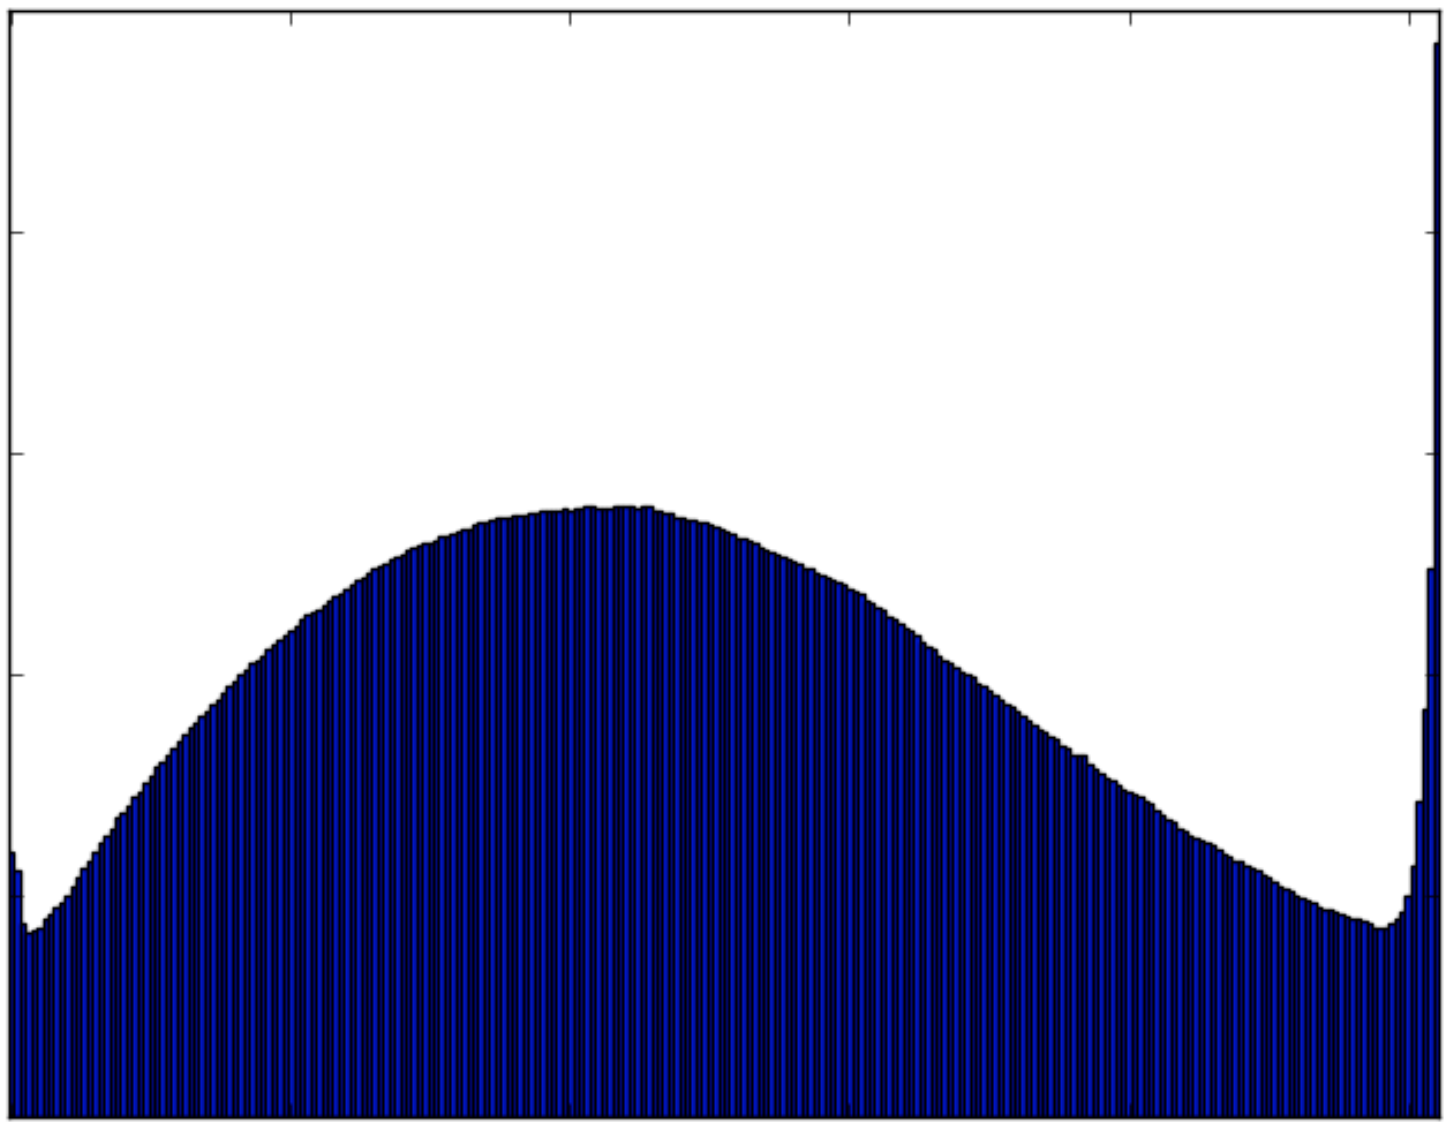
\includegraphics[width=0.6\linewidth,height=0.2\linewidth]{figs/CIFAR_pixel_distr}
		\end{figure}
	\end{block}
	\myfootnotewithlink{https://arxiv.org/abs/1701.05517}{Salimans T. et al. PixelCNN++: Improving the PixelCNN with Discretized Logistic Mixture Likelihood and Other Modifications, 2017}
\end{frame}
%=======
\subsection{Discretization of continuous distribution}
%=======
\begin{frame}{Discretization of continuous distribution}
	\vspace{-0.3cm}
	\begin{block}{Model discretization through CDF}
		\vspace{-0.6cm}
		\[
			F(\bx | \btheta) = \int_{-\infty}^{\bx} p(\bx' | \btheta) d\bx'; \quad 
			P(\by | \btheta) = F(\by + 0.5 | \btheta) - F(\by - 0.5 | \btheta)
		\]
	\end{block}
	\vspace{-0.6cm}
	\begin{block}{Mixture of logistic distributions}
		\vspace{-0.7cm}
		\[
			p(x | \mu, s) = \frac{\exp^{-(x - \mu) / s}}{s (1 + \exp^{-(x - \mu) / s})^2}; \quad p(x | \bpi, \bmu, \bs) = \sum_{k=1}^K \pi_k p(x | \mu_k, s_k).
		\]
		\vspace{-0.7cm}
	\end{block}
	\begin{block}{PixelCNN++}
		\vspace{-0.7cm}
		\[
			p(\bx | \btheta) = \prod_{j=1}^m p(x_j | \bx_{1:j-1}, \btheta); \quad p(x_j | \bx_{1:j-1}, \btheta) = \sum_{k=1}^K \pi_k p(x | \mu_k, s_k).
		\]
		\vspace{-0.5cm} \\
		Here, $\pi_k = \pi_{k, \btheta}(\bx_{1:j-1})$, $\mu_k = \mu_{k, \btheta}(\bx_{1:j-1})$, $s_k = s_{k, \btheta}(\bx_{1:j-1})$.
	\end{block}

	For the pixel edge cases of 0, replace $y - 0.5$ by $-\infty$, and for 255 replace $y + 0.5$ by $+\infty$.
	\myfootnotewithlink{https://arxiv.org/abs/1701.05517}{Salimans T. et al. PixelCNN++: Improving the PixelCNN with Discretized Logistic Mixture Likelihood and Other Modifications, 2017}\end{frame}
%=======
\subsection{Dequantization of discrete data}
%=======
\begin{frame}{Uniform dequantization}
	Let dequantize discrete distribution $\Pi(\by)$ to continuous distribution $\pi(\bx)$ in the following way: $\bx = \by + \bu$, where  $\bu \sim U[0, 1]$.
	\begin{minipage}{0.7\linewidth}	
		\begin{block}{Theorem}
			Fitting continuous model $p(\bx | \btheta)$ on uniformly dequantized data is equivalent to maximization of a lower bound on log-likelihood for a discrete model:
			\vspace{-0.2cm}
			\[
			P(\by | \btheta) = \int_{U[0, 1]} p(\by + \bu | \btheta) d \bu
			\]
			\vspace{-0.5cm} 
		\end{block}
	\end{minipage}%
	\begin{minipage}{0.3\linewidth}
		\begin{figure}
			\centering
			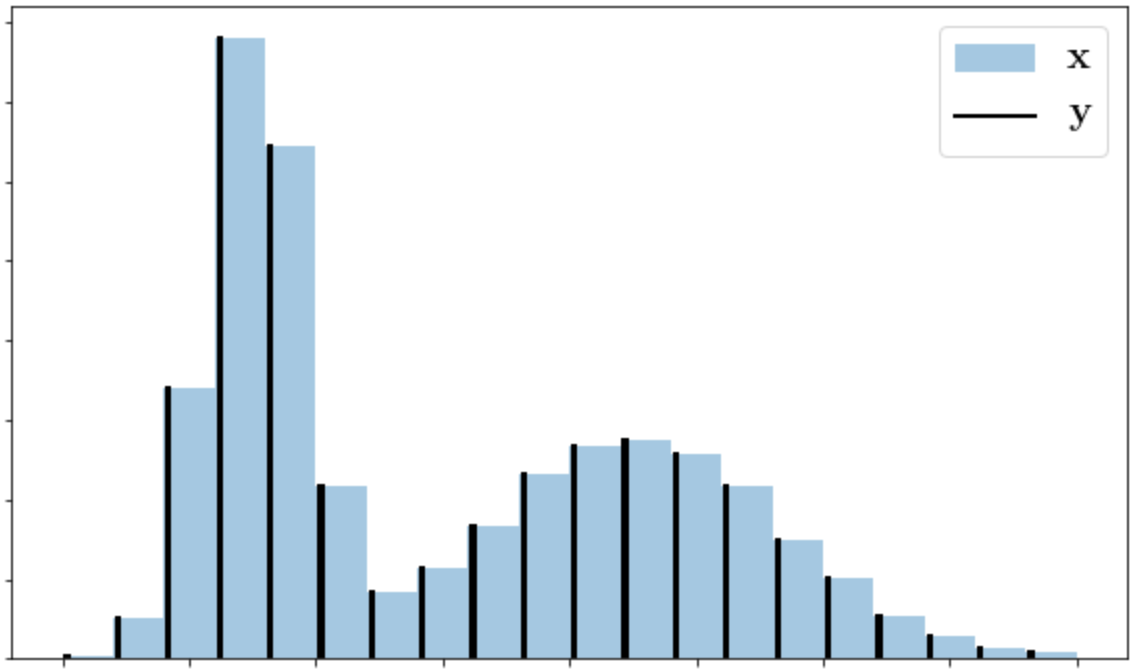
\includegraphics[width=\linewidth,height=0.8\linewidth]{figs/uniform_dequantization.png}
		\end{figure}
	\end{minipage}

	\begin{block}{Proof}
		\vspace{-0.8cm}
		{\small
		\begin{multline*}
			\bbE_{\pi} \log p(\bx | \btheta) = \int \pi(\bx) \log p(\bx | \btheta) d \bx = \sum \Pi(\by) \int_{U[0,1]} \log p(\by + \bu | \btheta) d \bu \leq \\
			\leq \sum \Pi(\by) \log \int_{U[0,1]}  p(\by + \bu | \btheta) d \bu = \\ = \sum \Pi(\by) \log P(\by | \btheta) = \bbE_{\Pi} \log P(\by | \btheta).
		\end{multline*}
		}
	\end{block}
	\myfootnotewithlink{https://arxiv.org/abs/1511.01844}{Theis L., Oord A., Bethge M. A note on the evaluation of generative models. 2015}
\end{frame}
%=======
\begin{frame}{Variational dequantization}
	\begin{minipage}[t]{0.5\columnwidth}
		\begin{figure}
			\centering
			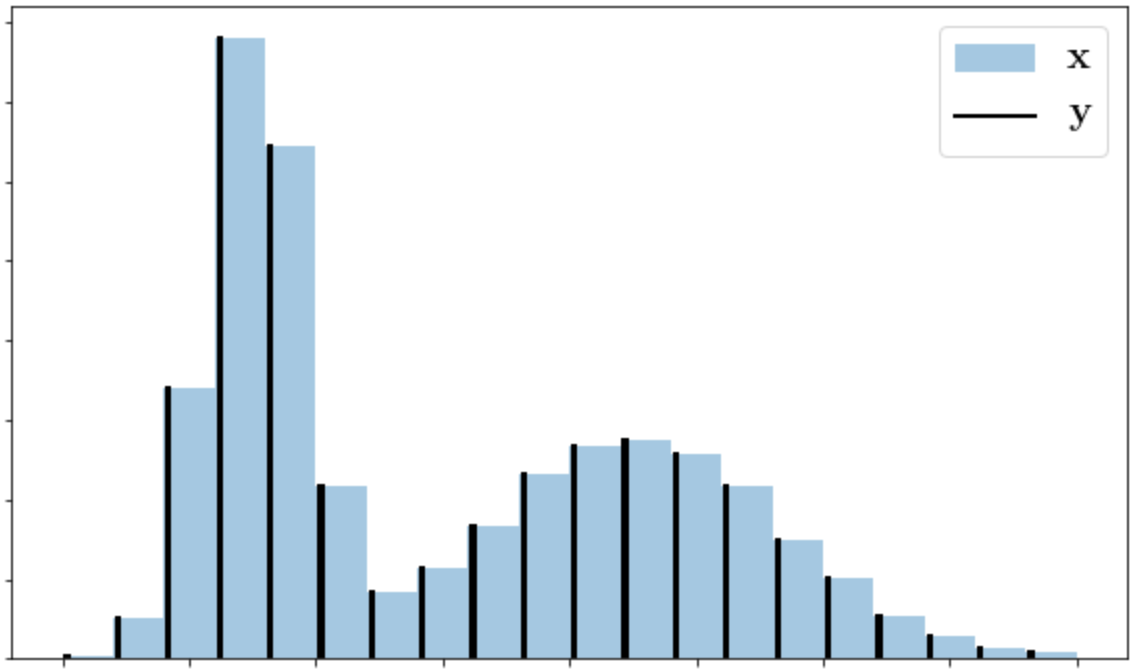
\includegraphics[width=0.8\linewidth]{figs/uniform_dequantization.png}
		\end{figure}
	\end{minipage}%
	\begin{minipage}[t]{0.5\columnwidth}
		\begin{figure}
			\centering
			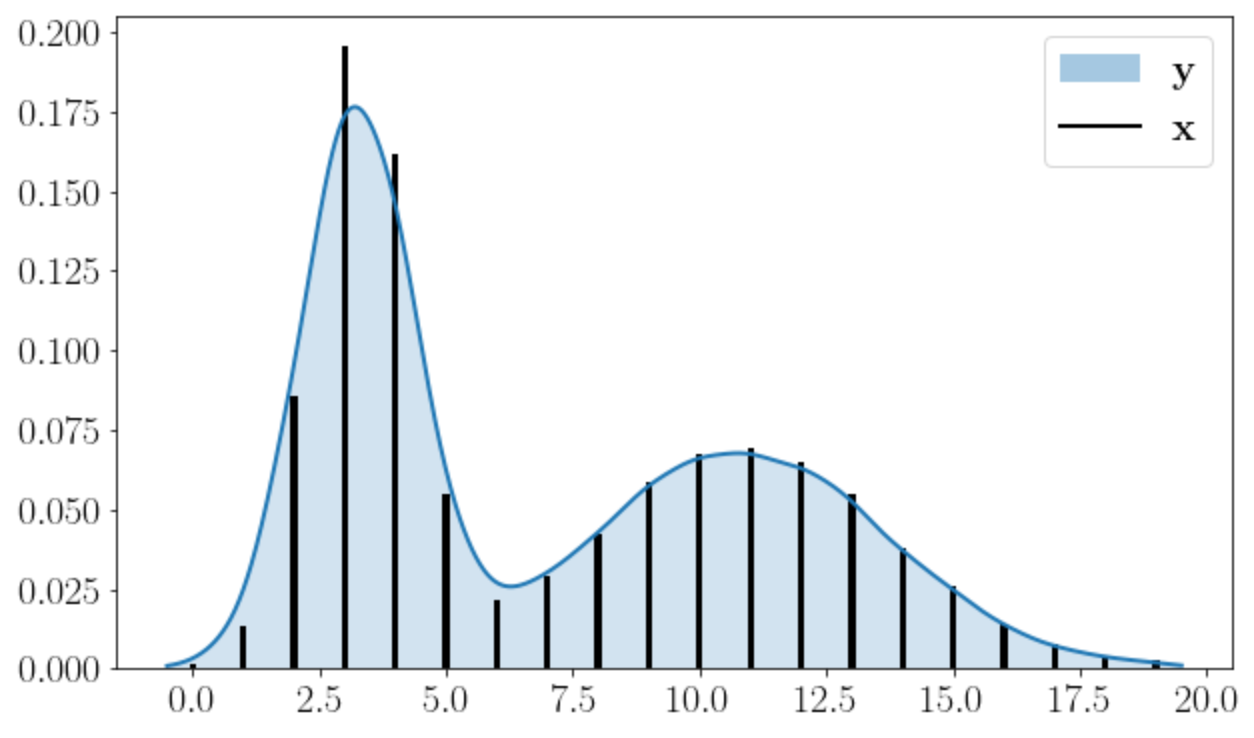
\includegraphics[width=0.8\linewidth]{figs/variational_dequantization.png}
		\end{figure}
	\end{minipage}
	\begin{itemize}
		\item $p(\bx | \btheta)$ assign uniform density to unit hypercubes $\by + U[0, 1]$ (left fig).
		\item Smooth dequantization is more natural (right fig).
		\item Neural network density models are smooth function approximators.
	\end{itemize}
	Introduce variational dequantization noise distribution $q(\bu | \by)$, which tells what kind of noise we have to add to our discrete data.  \\
	Treat it as an approximate posterior as in VAE model. 
\end{frame}
%=======
\begin{frame}{Variational dequantization}
	\vspace{-0.2cm}
	\begin{block}{Variational lower bound}
		\vspace{-0.7cm}
		\begin{multline*}
			\log P(\by | \btheta) = \left[ \log \int q(\bu | \by) \frac{p(\by + \bu | \btheta)}{q(\bu | \by)} d \bu \right] \geq \\ 
			\geq  \int q(\bu | \by) \log \frac{p(\by + \bu | \btheta)}{q(\bu | \by)} d \bu = \mathcal{L}(q, \btheta).
		\end{multline*}
		\vspace{-0.6cm}
	\end{block}
	Uniform dequantization is a special case of variational dequantization ($q(\bu | \by) = U[0, 1]$).
	\begin{block}{Flow++: flow-based variational dequantization}
		Let $\bu = g(\bepsilon, \by, \blambda)$ is a flow model with base distribution $\bepsilon \sim p(\bepsilon)$:
		\vspace{-0.3cm}
		\[
		q(\bu | \by) = p(f(\bu, \by, \blambda)) \cdot \left| \det \frac{\partial f(\bu, \by, \blambda)}{\partial \bu}\right|.
		\]
		\vspace{-0.3cm}
		\[
		\log P(\by | \btheta) \geq \cL(\blambda, \btheta) = \int p(\bepsilon) \log \left( \frac{p(\by + g(\bepsilon, \by, \blambda) | \btheta)}{p(\bepsilon) \cdot \left| \det \bJ_g\right|^{-1}} \right) d\bepsilon.
		\]
		\vspace{-0.3cm}
	\end{block}
	\myfootnotewithlink{https://arxiv.org/abs/1902.00275}{Ho J. et al. Flow++: Improving Flow-Based Generative Models with Variational Dequantization and Architecture Design, 2019}
\end{frame}
%=======
\section{ELBO surgery}
%=======
\begin{frame}{ELBO surgery}
	\vspace{-0.3cm}
	\[
	    \frac{1}{n} \sum_{i=1}^n \mathcal{L}_i(q, \btheta) = \frac{1}{n} \sum_{i=1}^n \Bigl[ \mathbb{E}_{q(\bz | \bx_i)} \log p(\bx_i | \bz, \btheta) - KL(q(\bz | \bx_i) || p(\bz)) \Bigr].
	\]
	\vspace{-0.3cm}
	\begin{block}{Theorem}
		\[
		    \frac{1}{n} \sum_{i=1}^n KL(q(\bz | \bx_i) || p(\bz)) = {\color{violet} KL(q_{\text{agg}}(\bz) || p(\bz))} + {\color{teal}\bbI_{q} [\bx, \bz]};
		\]
		\begin{itemize}
			\item $q_{\text{agg}}(\bz) = \frac{1}{n} \sum_{i=1}^n q(\bz | \bx_i)$ -- \textbf{aggregated} posterior distribution.
			\item $\bbI_{q} [\bx, \bz]$ -- mutual information between $\bx$ and $\bz$ under empirical data distribution and distribution $q(\bz | \bx)$.
			\item  {\color{violet} First term} pushes $q_{\text{agg}}(\bz)$ towards the prior $p(\bz)$.
			\item {\color{teal}Second term} reduces the amount of	information about $\bx$ stored in $\bz$. 
		\end{itemize}
	\end{block}
	\myfootnotewithlink{http://approximateinference.org/accepted/HoffmanJohnson2016.pdf}{Hoffman M. D., Johnson M. J. ELBO surgery: yet another way to carve up the variational evidence lower bound, 2016}
\end{frame}
%=======
\begin{frame}{ELBO surgery}
	\begin{block}{Theorem}
		\vspace{-0.3cm}
		\[
		    \frac{1}{n} \sum_{i=1}^n KL(q(\bz | \bx_i) || p(\bz)) = KL(q_{\text{agg}}(\bz) || p(\bz)) + \bbI_q [\bx, \bz].
		\]
		\vspace{-0.4cm}
	\end{block}
	\begin{block}{Proof}
		\vspace{-0.5cm}
		{\footnotesize
		\begin{multline*}
		    \frac{1}{n} \sum_{i=1}^n KL(q(\bz | \bx_i) || p(\bz)) = \frac{1}{n} \sum_{i=1}^n \int q(\bz | \bx_i) \log \frac{q(\bz | \bx_i)}{p(\bz)} d \bz = \\
		    = \frac{1}{n} \sum_{i=1}^n \int q(\bz | \bx_i) \log \frac{{\color{violet}q_{\text{agg}}(\bz)} {\color{teal}q(\bz | \bx_i)}}{{\color{violet}p(\bz)} {\color{teal}q_{\text{agg}}(\bz)}} d \bz 
		    = \int \frac{1}{n} \sum_{i=1}^n  q(\bz | \bx_i) \log {\color{violet}\frac{q_{\text{agg}}(\bz)}{p(\bz)}} d \bz + \\ 
		    + \frac{1}{n}\sum_{i=1}^n \int q(\bz | \bx_i) \log {\color{teal}\frac{q(\bz | \bx_i)}{q_{\text{agg}}(\bz)}} d \bz = 
		     KL (q_{\text{agg}}(\bz) || p(\bz)) + \frac{1}{n}\sum_{i=1}^n KL(q(\bz | \bx_i) || q_{\text{agg}}(\bz))
		\end{multline*}
		}
		Without proof:
		\vspace{-0.4cm}
		\[
			\bbI_{q} [\bx, \bz] = \frac{1}{n}\sum_{i=1}^n KL(q(\bz | \bx_i) || q_{\text{agg}}(\bz)) \in [0, \log n].
		\]
	\end{block}

	\myfootnotewithlink{http://approximateinference.org/accepted/HoffmanJohnson2016.pdf}{Hoffman M. D., Johnson M. J. ELBO surgery: yet another way to carve up the variational evidence lower bound, 2016}
\end{frame}
%=======
\begin{frame}{ELBO surgery}
	\begin{block}{ELBO revisiting}
		\vspace{-0.7cm}
		\begin{multline*}
		    \frac{1}{n}\sum_{i=1}^n \cL_i(q, \btheta) = \frac{1}{n} \sum_{i=1}^n \left[ \mathbb{E}_{q(\bz | \bx_i)} \log p(\bx_i | \bz, \btheta) - KL(q(\bz | \bx_i) || p(\bz)) \right] = \\
		    = \underbrace{\frac{1}{n} \sum_{i=1}^n \mathbb{E}_{q(\bz | \bx_i)} \log p(\bx_i | \bz, \btheta)}_{\text{Reconstruction loss}} - \underbrace{\vphantom{ \sum_{i=1}^n} \bbI_q [\bx, \bz]}_{\text{MI}} - \underbrace{\vphantom{ \sum_{i=1}^n} KL(q_{\text{agg}}(\bz) || {\color{teal}p(\bz)})}_{\text{Marginal KL}}
		\end{multline*}
		\vspace{-0.3cm}
	\end{block}
	Prior distribution $p(\bz)$ is only in the last term.
	\begin{block}{Optimal VAE prior}
		\vspace{-0.7cm}
		\[
	  		KL(q_{\text{agg}}(\bz) || p(\bz)) = 0 \quad \Leftrightarrow \quad p (\bz) = q_{\text{agg}}(\bz) = \frac{1}{n} \sum_{i=1}^n q(\bz | \bx_i).
		\]
		\vspace{-0.4cm} \\
		The optimal prior $p(\bz)$ is the aggregated posterior $q_{\text{agg}}(\bz)$!
	\end{block}
	
	\myfootnotewithlink{http://approximateinference.org/accepted/HoffmanJohnson2016.pdf}{Hoffman M. D., Johnson M. J. ELBO surgery: yet another way to carve up the variational evidence lower bound, 2016}
\end{frame}
%=======
\section{VAE limitations}
%=======
\subsection{VAE prior}
%=======
\begin{frame}{VAE limitations}
	\begin{itemize}
		\item Poor generative distribution (decoder)
		\[
		p(\bx | \bz, \btheta) = \mathcal{N}(\bx| \bmu_{\btheta}(\bz), \bsigma^2_{\btheta}(\bz)) \quad \text{or } = \text{Softmax}(\bpi_{\btheta}(\bz)).
		\]
		\item Loose lower bound
		\[
		\log p(\bx | \btheta) - \mathcal{L}(q, \btheta) = (?).
		\]
		\item \textbf{Poor prior distribution}
		\[
		p(\bz) = \mathcal{N}(0, \mathbf{I}).
		\]
		\item Poor variational posterior distribution (encoder)
		\[
		q(\bz | \bx, \bphi) = \mathcal{N}(\bz| \bmu_{\bphi}(\bx), \bsigma^2_{\bphi}(\bx)).
		\]
	\end{itemize}
\end{frame}
%=======
\begin{frame}{Optimal VAE prior}
	\begin{itemize}
		\item Standard Gaussian $p(\bz) = \mathcal{N}(0, I)$ $\Rightarrow$ over-regularization;
		\item $p(\bz) = q_{\text{agg}}(\bz) = \frac{1}{n}\sum_{i=1}^n q(\bz | \bx_i)$ $\Rightarrow$ overfitting and highly expensive.
	\end{itemize}
	\vspace{-0.5cm}
	\begin{minipage}[t]{0.5\columnwidth}
		\begin{block}{Non learnable prior $p(\bz)$}
			\begin{figure}[h]
				\centering
				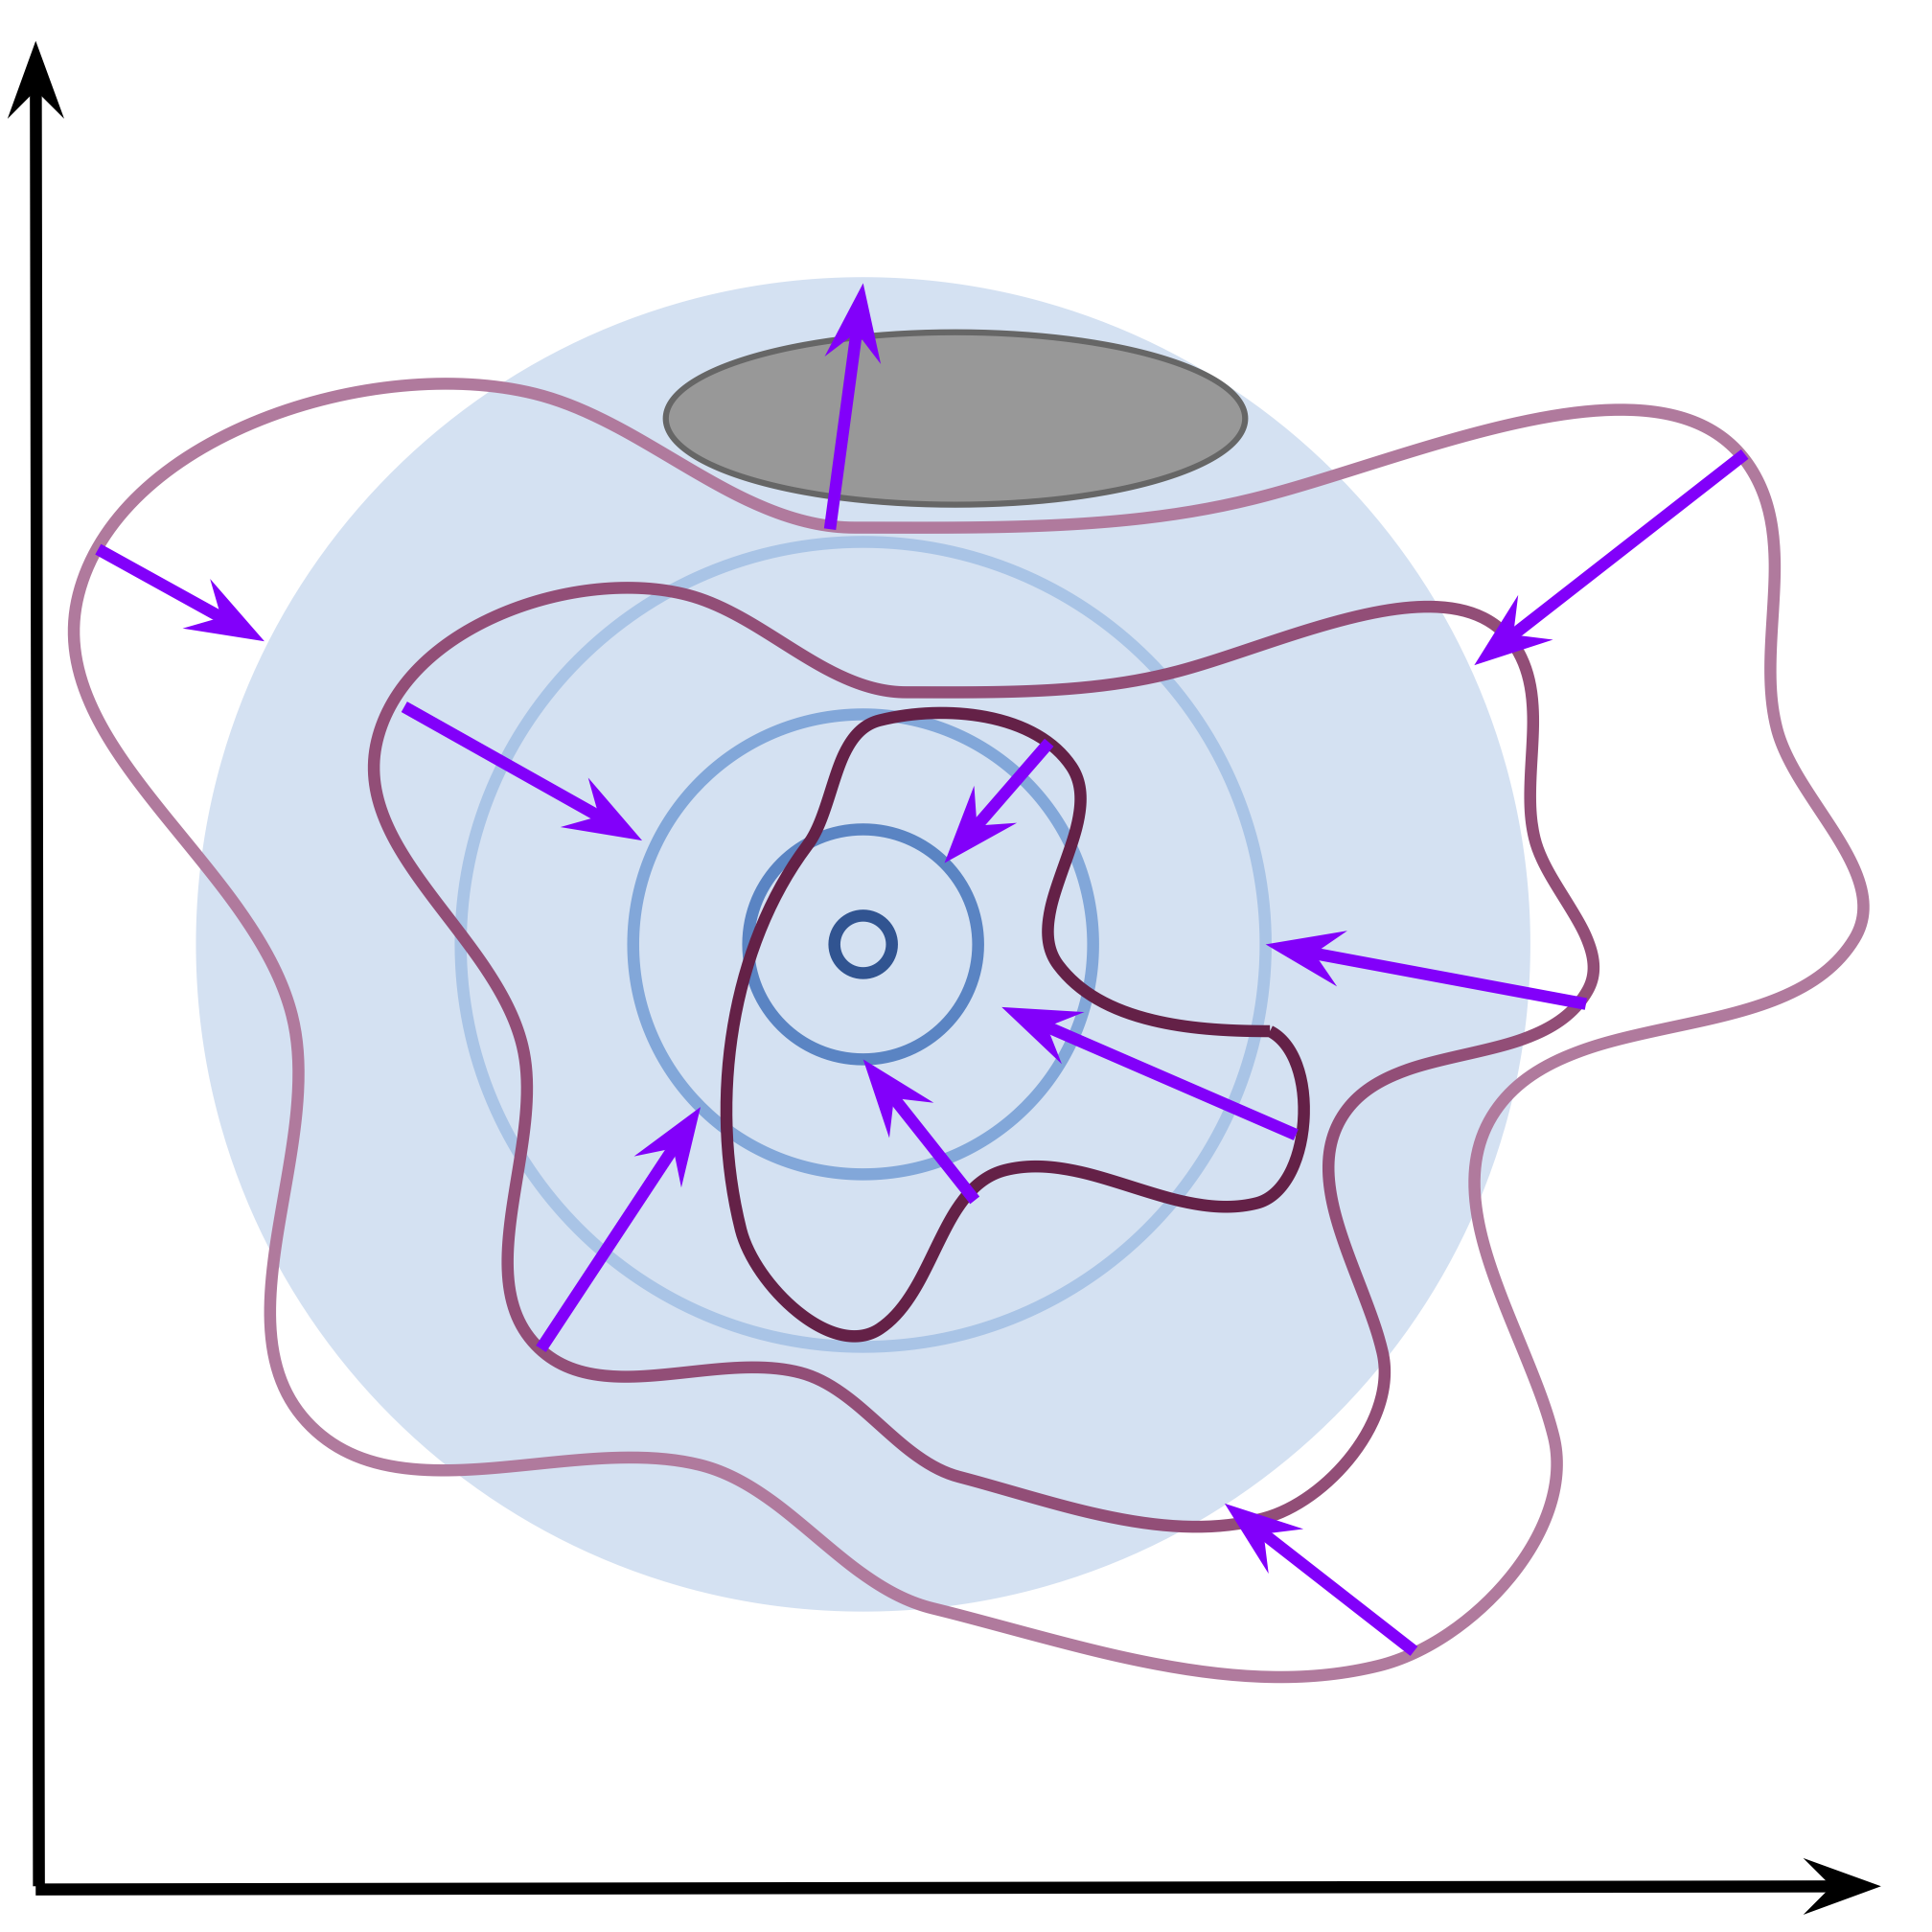
\includegraphics[width=0.6\linewidth]{figs/non_learnable_prior}
			\end{figure}
		\end{block}
	\end{minipage}%
	\begin{minipage}[t]{0.5\columnwidth}
		\begin{block}{Learnable prior $p(\bz | \blambda)$}
			\begin{figure}[h]
				\centering
				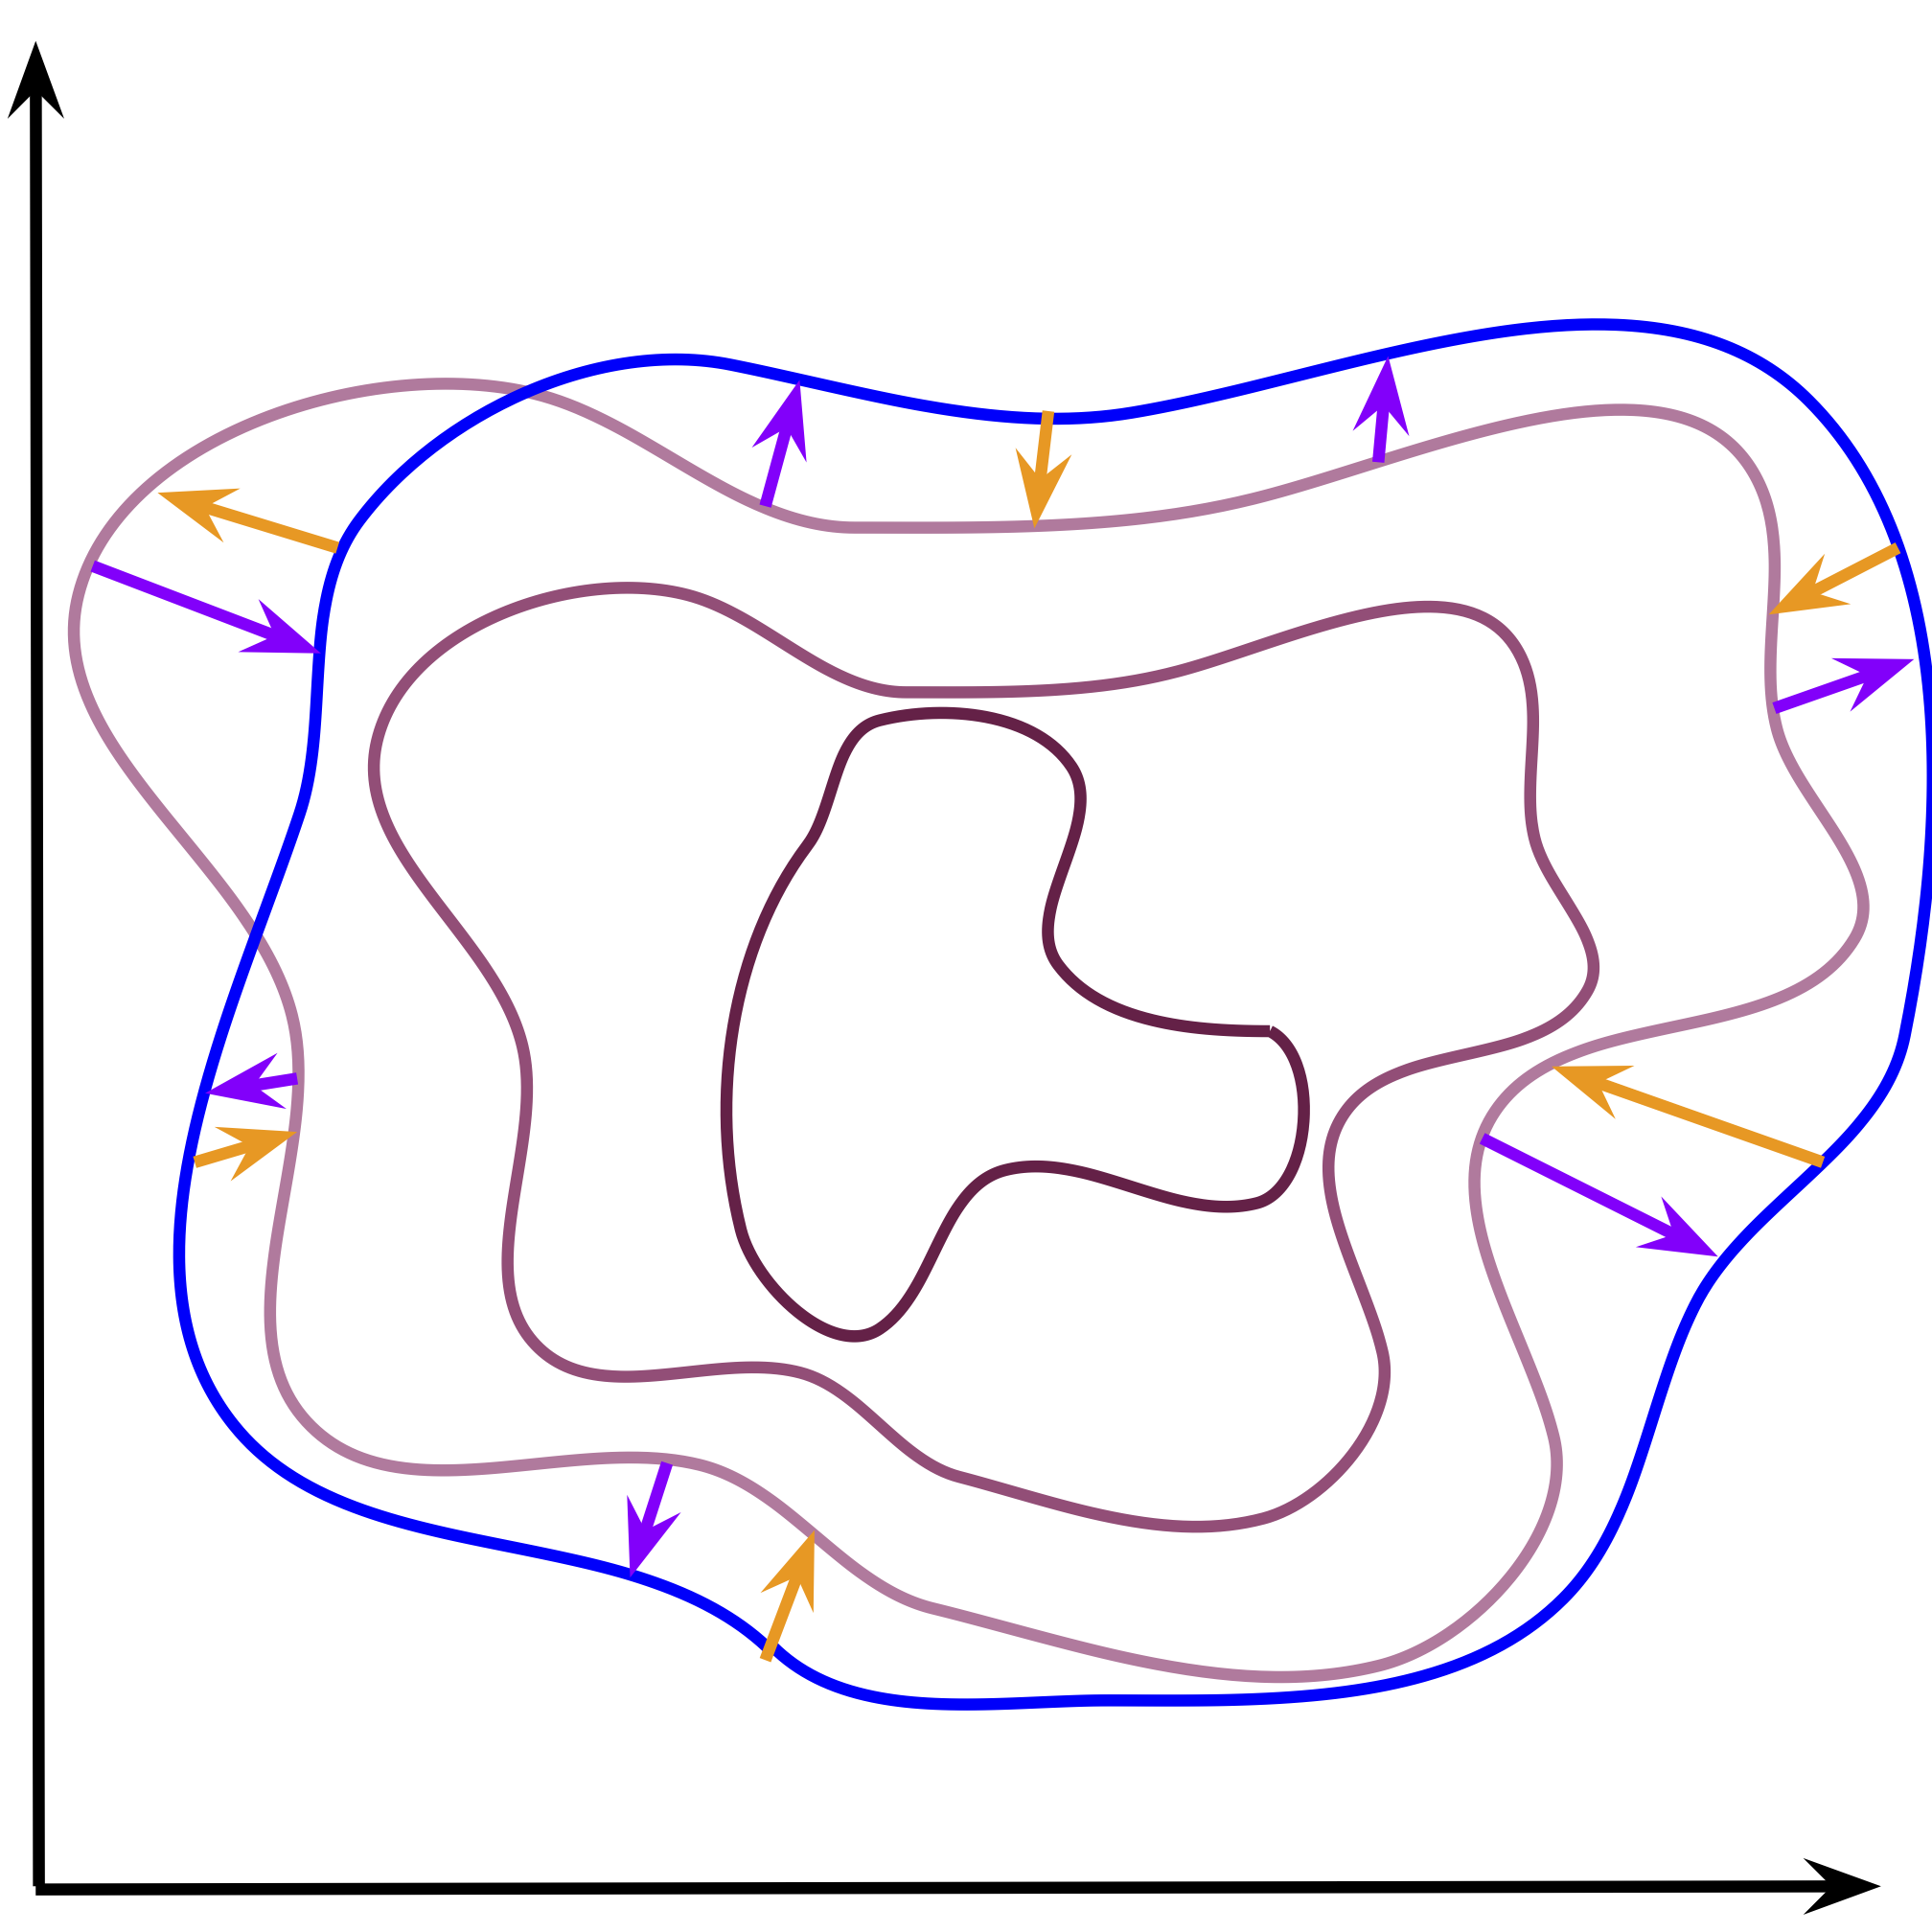
\includegraphics[width=0.6\linewidth]{figs/learnable_prior}
			\end{figure}
		\end{block}
	\end{minipage}
	\vspace{-0.4cm}
	\begin{block}{ELBO revisiting}
		\vspace{-0.3cm}
		\[
			\frac{1}{n}\sum_{i=1}^n \cL_i(q, \btheta) = \text{RL} - \text{MI} -  KL(q_{\text{agg}}(\bz) || {\color{teal}p(\bz | \blambda)})
		\]
		It is Forward KL with respect to $p(\bz | \blambda)$.
	\end{block}
	\myfootnotewithlink{https://jmtomczak.github.io/blog/7/7\_priors.html}{image credit: https://jmtomczak.github.io/blog/7/7\_priors.html}
\end{frame}
%=======
\begin{frame}{Flow-based VAE prior}
	\begin{block}{Flow model in latent space}
		\vspace{-0.5cm}
		\[
			\log p(\bz | \blambda) = \log p(\bz^*) + \log  \left | \det \left(\frac{d \bz^*}{d\bz}\right)\right| = \log p(f(\bz, \blambda)) + \log \left | \det (\bJ_f)\right| 
		\]
		\vspace{-0.3cm}
		\[
			\bz = g(\bz^*, \blambda) = f^{-1}(\bz^*, \blambda)
		\]
	\end{block}
	\vspace{-0.3cm}
	\begin{itemize}
		\item RealNVP with coupling layers.
		\item Autoregressive flow (fast $f(\bz, \blambda)$, slow $g(\bz^*, \blambda)$).
		\item {\color{gray}Is it OK to use IAF for VAE prior?}
	\end{itemize}
	\begin{block}{ELBO with flow-based VAE prior}
		\vspace{-0.5cm}
		{\small
		\begin{multline*}
			\mathcal{L}(\bphi, \btheta) = \mathbb{E}_{q(\bz | \bx, \bphi)} \left[ \log p(\bx | \bz, \btheta) + {\color{violet}\log p(\bz | \blambda)} - \log q(\bz | \bx, \bphi) \right] \\
				= \mathbb{E}_{q(\bz | \bx, \bphi)} \Bigl[ \log p(\bx | \bz, \btheta) + \underbrace{ \Bigl({\color{violet} \log p(f(\bz, \blambda)) + \log \left| \det (\bJ_f) \right|} \Bigr) }_{\text{flow-based prior}} - \log q(\bz | \bx, \bphi) \Bigr] 
		\end{multline*}
		}
		{\color{gray}Is it possible to use non-invertible model in VAE prior?}
	\end{block}
	\myfootnotewithlink{https://arxiv.org/abs/1611.02731}{Chen X. et al. Variational Lossy Autoencoder, 2016}
\end{frame}
%=======
\subsection{VAE posterior}
%=======
\begin{frame}{VAE limitations}
	\begin{itemize}
		\item Poor generative distribution (decoder)
		\[
		p(\bx | \bz, \btheta) = \mathcal{N}(\bx| \bmu_{\btheta}(\bz), \bsigma^2_{\btheta}(\bz)) \quad \text{or } = \text{Softmax}(\bpi_{\btheta}(\bz)).
		\]
		\item Loose lower bound
		\[
		\log p(\bx | \btheta) - \mathcal{L}(q, \btheta) = (?).
		\]
		\item Poor prior distribution
		\[
		p(\bz) = \mathcal{N}(0, \mathbf{I}).
		\]
		\item \textbf{Poor variational posterior distribution (encoder)}
		\[
		q(\bz | \bx, \bphi) = \mathcal{N}(\bz| \bmu_{\bphi}(\bx), \bsigma^2_{\bphi}(\bx)).
		\]
	\end{itemize}
\end{frame}
%=======
\begin{frame}{Variational posterior}
	\begin{block}{ELBO decomposition}
		\[
		\log p(\bx | \btheta) = \mathcal{L}(q, \btheta) + KL(q(\bz | \bx, \bphi) || p(\bz | \bx, \btheta)).
		\]
	\end{block}
	\begin{itemize}
		\item E-step of EM-algorithm: $KL(q(\bz | \bx, \bphi) || p(\bz | \bx, \btheta)) = 0$. \\
		(In this case the lower bound is tight $\log p(\bx | \btheta) = \mathcal{L}(q, \btheta)$). \\
		\item $q(\bz | \bx, \bphi) = \mathcal{N}(\bz| \bmu_{\bphi}(\bx), \bsigma^2_{\bphi}(\bx))$ is a unimodal distribution (not expressive enough). \\
		\item NF convert a simple distribution to a complex one. Let use NF in VAE posterior.
	\end{itemize}
	Apply a sequence of transformations to the random variable
	\[
		\bz \sim q(\bz | \bx, \bphi) = \mathcal{N}(\bz| \bmu_{\bphi}(\bx), \bsigma^2_{\bphi}(\bx)).
	\]
	Let $q(\bz | \bx, \bphi)$ (VAE encoder) be a base distribution for a flow model.
\end{frame}
%=======
\begin{frame}{Summary}
	\begin{itemize}
		\item Lots of data are discrete. We able to discretize the model or to dequantize our data to use continuous model.
		\vfill
		\item Uniform dequantization is the simplest form of dequantization. Variational dequantization is a more natural type that uses variational inference.
		\vfill
		\item The ELBO surgery reveals insights about a prior distribution in VAE. The optimal prior is the aggregated posterior.
		\vfill
		\item We could use flow-based prior in VAE (even autoregressive).
		\vfill
		\item We could use flows to make variational posterior more expressive. 
	\end{itemize}
\end{frame}

\end{document} 